% Ubah judul dan label berikut sesuai dengan yang diinginkan.
\section{Architecture}
\label{sec:arsitektur}

% Ubah paragraf-paragraf pada bagian ini sesuai dengan yang diinginkan.

\subsection{Retriever}
\label{subsec:Retriever}

Before using data for the language model, it is necessary to search for relevant data. To perform this data search, searches are conducted by looking at the location of the data within the vector. For this, data must be converted into a vector format that can be computed. There are many methods for doing this, such as \emph{one-hot}, \emph{Word2Vec}, and \emph{Doc2Vec}. These methods provide effective pathways for text quantification but often ignore contextual information. The \emph{Transformer} model, introduced by Google in 2017, overcomes the shortcomings of existing text quantification methods and is built using unsupervised training on large volumes of unlabeled corpus data \cite{vaswani2017attention}. The \emph{Transformer} is a neural network architecture widely used in NLP, text classification, question-answering systems, and more. This model consists of several \emph{encoders} and \emph{decoders}, each composed of several layers of identical blocks. These blocks are stacked together to form the overall \emph{Transformer} architecture \cite{miao2016processing}. The structure of the \emph{transformer} can be seen in Figure \ref*{fig:transformer}.

\begin{figure*}
  \centering
  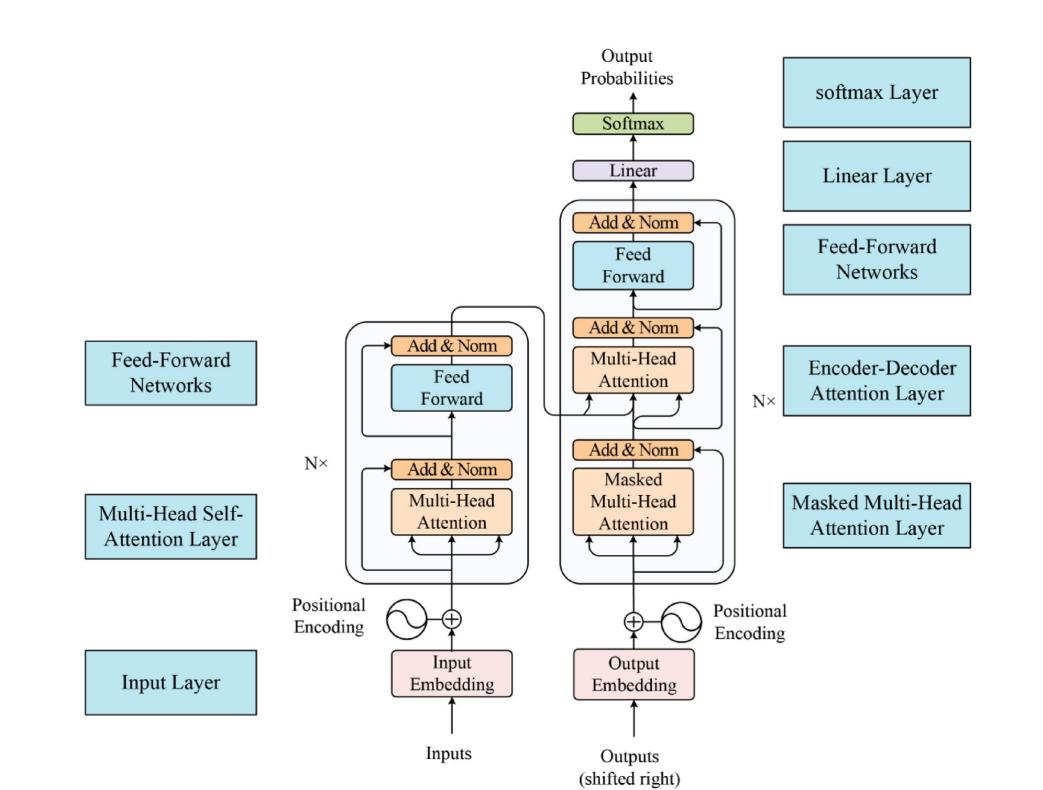
\includegraphics[width=.6\textwidth]{gambar/struktur-transformer.jpg}
  \caption{Transformer structure \cite{vaswani2017attention}}
  \label{fig:transformer}
\end{figure*}

In the \emph{transformer} architecture, there are two main components: the \emph{encoder} and the \emph{decoder}, each consisting of a series of identical layers. Each layer in the \emph{encoder} and \emph{decoder} has two sub-layers, namely the \emph{multi-head attention} mechanism and the \emph{fully connected network}. \emph{Multi-head attention} allows the model to process parts of the data in parallel and integrate information from various positions within the data. Furthermore, the \emph{transformer} features a \emph{self-attention} mechanism, which allows each output from the \emph{encoder} or \emph{decoder} to consider all previous inputs. This differs from other algorithms that are limited by the distance between relevant inputs and outputs. This mechanism also aids in understanding long-term dependencies in text, which is crucial for tasks such as translation. \emph{Positional encoding} is used to provide positional information to the model, as the \emph{transformer} model lacks recursion or convolution that naturally captures the sequence of information \cite{vaswani2017attention}.
 

\subsection{Augment and Generation}
\label{subsec:AugmentGeneration}

During the \emph{augmentation} process, the LLM model will operate by processing the \emph{prompt} from the user using the context already obtained from the previous \emph{retriever} process \cite{bansal2024llm}. The tool is implemented by first creating a backend system using LangChain to connect various modules and LLM processes. LangChain serves as a connector to various other modules. Subsequently, a selection of the LLM framework to be used is made. The framework employed must be \emph{open-source} and lightweight in order to be effective in use. Therefore, in the testing phase, trials will be conducted on various frameworks to test the effectiveness of these frameworks. Some to be tested include RASA, Hugging Face, and Ilama Cpp. Testing is conducted by evaluating the performance of each framework, as well as considering their advantages and disadvantages. After that, the most effective framework will be selected for use in implementing this tool.

During the \emph{generation} process, the LLM model will produce output in the form of answers to the questions provided by the user. This output will be given to the user as an answer to their question. In this process, the LLM model will utilize the context obtained from the previous \emph{retriever} process. Thus, the LLM model will be able to provide answers that are more relevant and accurate. The testing used the following configuration:
\begin{lstlisting}[
  language=python,
  caption={Test configuration},
]
model = AutoModelForCausalLM.from_pretrained(
   "$MODEL_NAME",
    load_in_8bit=True,
)
pipeline = pipeline(
    "text-generation",
    model=model,
    return_full_text=False,
    tokenizer=tokenizer,
    max_new_tokens=512,
     do_sample=True,
    pad_token_id=tokenizer.eos_token_id
)
\end{lstlisting}

After that, an analysis is conducted on the results obtained from the LLM model. The results will be analyzed based on the relevance and accuracy of the answers provided. This is done by comparing the answers with the answers from the data source. For example, for the question: "What should be done in the event of a power outage?" the relevant answer according to the book is "In the event of a power outage, do not panic, the emergency generator will restore power shortly, find out the problem and reason for the power outage, inform the authorities...". Furthermore, an analysis is conducted on the use of RAM and VRAM. This is done to determine how efficient the LLM model is in using resources. Thus, it can be determined how effective the LLM model is in providing answers that are relevant, accurate, and efficient.


% Contoh input gambar pada kolom.
% \begin{figure} [ht]
%   \centering
%   % Ubah sesuai dengan nama file gambar dan ukuran yang akan digunakan.
%   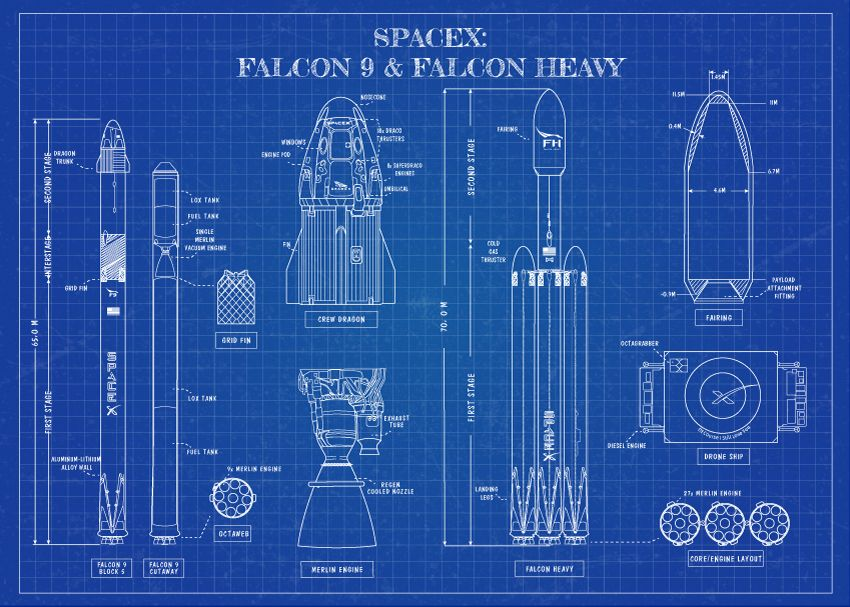
\includegraphics[width=0.4\textwidth]{gambar/cetakbiru.jpg}

%   % Ubah sesuai dengan keterangan gambar yang diinginkan.
%   \caption{Cetak biru roket yang akan diuji coba. \cite{cetakbiruspacex}}
%   \label{fig:cetakbiru}
% \end{figure}

% \lipsum[9-10]

% \subsection{Lorem Ipsum}
% \label{subsec:loremipsum}

% \lipsum[11]

% % Contoh pembuatan tabel.
% \begin{table}
%   \caption{Contoh tabel sederhana}
%   \label{tab:tabelsederhana}
%   \centering
%   \begin{tabular}{lll}
%     \toprule
%     Heading1 & Heading2 & Heading3  \\
%     \midrule
%     One      & Two      & Three     \\
%     Four     & Five     & Six       \\
%     \bottomrule
%   \end{tabular}
% \end{table}

% % Contoh pembuatan potongan kode.
% \begin{lstlisting}[
%   language=C++,
%   caption={Program halo dunia.},
%   label={lst:halodunia}
% ]
% #include <iostream>

% int main() {
%     std::cout << "Halo Dunia!";
%     return 0;
% }
% \end{lstlisting}

% \lipsum[12]

% % Contoh pembuatan daftar.
% \begin{enumerate}
%   \item \lipsum[13][1-4]
%   \item \lipsum[13][5-8]
%   \item \lipsum[13][9-12]
% \end{enumerate}

% \lipsum[14-15]
